\section[Wykład 4: 16-III-2017 - Temat: Algebraiczna teoria grafów.]{Temat: Algebraiczna teoria grafów.}
\subsection{Reprezentacja grafu}
\begin{definition}[Macierz przyległości] Macierzą przyległości graf $G=(V,E)$ , gdzie $V=\{1,2,..,n\},\; |V|=n$ to macierz $A\in M_{n\times m}$
$$A=[a_{ij}]_{n\times m}\text{, gdzie } a_{ij}=\left\{\begin{matrix}
1 & \text{jeżeli } \{i,j\}\in E\\
0 & \text{w pozostałych przypadkach}
\end{matrix}\right.$$
\end{definition}
\begin{example*}
\begin{multicols}{2}
$K_3$: 
\begin{figure}[H]
\centering
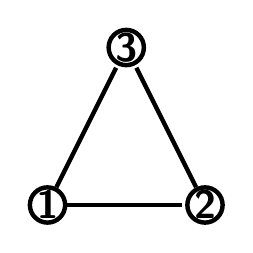
\begin{tikzpicture}[shorten >=1pt, auto, node distance=3cm, ultra thick,main node/.style={circle,draw,minimum size=.4cm,inner sep=0pt]}]%fill=black,
\begin{scope}[every node/.style={font=\sffamily\Large\bfseries}]
\node[main node] (v1) at (0,0) {1};
\node[main node] (v2) at (2,0) {2};
\node[main node] (v3) at (1,2) {3};
%\node[main node] (v) at (,) {};
\end{scope}
\begin{scope}
\draw  (v1) edge node{} (v2);
\draw  (v1) edge node{} (v3);
\draw  (v2) edge node{} (v3);
%\draw  (v) edge node{} (v);
\end{scope}
\end{tikzpicture}
\end{figure}
$$A(K_3)=\left [\begin{matrix}
0 & 1 & 1\\
1&0&1\\
1&1&0
\end{matrix}\right ]$$
\end{multicols}
\begin{multicols}{2}
$C_4$:
\begin{figure}[H]
\centering
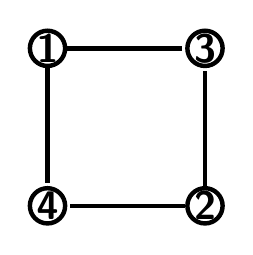
\begin{tikzpicture}[shorten >=1pt, auto, node distance=3cm, ultra thick,main node/.style={circle,draw,minimum size=.4cm,inner sep=0pt]}]%fill=black,
\begin{scope}[every node/.style={font=\sffamily\Large\bfseries}]
\node[main node] (v1) at (0,0) {1};
\node[main node] (v2) at (2,-2) {2};
\node[main node] (v3) at (2,0) {3};
\node[main node] (v4) at (0,-2) {4};
%\node[main node] (v) at (,) {};
\end{scope}
\begin{scope}
\draw  (v1) edge node{} (v4);
\draw  (v1) edge node{} (v3);
\draw  (v2) edge node{} (v3);
\draw  (v2) edge node{} (v4);
%\draw  (v) edge node{} (v);
\end{scope}
\end{tikzpicture}
\end{figure}
$$A(C_4)=\begin{bmatrix}
0 & 0 & 1 & 1\\ 
0 & 0 & 1 & 1\\ 
1 & 1 & 0 & 0\\ 
1 & 1 & 0 & 0
\end{bmatrix}$$
\end{multicols}
\end{example*}

\subsection{Operacje na macierzach}
\subsubsection{Dodawanie / Odejmowanie macierzy}
$$A_{m,n} \pm B_{m,n} = C_{m,n} \overset{def.}{\longrightarrow} c_{i,j}=a_{i,j}\pm b_{i,j}$$
\subsubsection{Mnożenie}
$$A_{m,n} * B_{n,o} = C_{m,o} \overset{def.}{\longrightarrow} c_{i,j}= \sum_{k=1}^n a_{i,k} * b_{k,j}$$
Przykład:
$$\begin{bmatrix}
1 & 2 & 3\\ 
3 & 2 & 1
\end{bmatrix} * \begin{bmatrix}
1 & -2\\ 
3 & 2\\ 
0 & 4
\end{bmatrix}=\begin{bmatrix}
1*1+2*3+3*0 & 1+*-2+2*2+3*4\\ 
3*1+2*3+1*0 & 3*-2+2*2+1*4
\end{bmatrix} = \begin{bmatrix}
7&14\\
9&2
\end{bmatrix}$$
\textbf{Mnożenie macierzy nie jest przemienne!}
\subsubsection{Transpozycja macierzy}
\begin{definition}[Macierz transponowana]
Macierz transponowaną względem macierzy $A_{m,n}$ nazywa się taką macierz $A_{n,m}^T$ w której wiersze odpowiadają kolumnom macierzy $A_{m,n}$/
\end{definition}
$$A=\begin{bmatrix}
1 & 2& 3\\
4& 5 &6
\end{bmatrix}\ A^T=\begin{bmatrix}
1 & 4\\
2 & 5\\
3 & 6
\end{bmatrix}\ A=(A^T)^T$$

\subsubsection{Wyznacznik}
własności:
\begin{itemize}
\item Jeśli wyznacznik ma dwie takie same kolumny / wiersze wyznacznik jest równy 0
\item Jeżeli w wyznaczniku do elementów jednego wiersza (lub kolumny) dodamy lub odejmiemy dowolną kombinację liniową innych wierszy lub kolumn to wartość wyznacznika nie zmieni się.
\end{itemize}
\paragraph{Macierz $3\times 3$}
$$\begin{vmatrix}
a_1&a_2&a_3\\
b_1&b_2&b_3\\
c_1&c_2&c_3
\end{vmatrix}=\begin{vmatrix}
a_1&a_2&a_3\\
b_1&b_2&b_3\\
c_1&c_2&c_3
\end{vmatrix}\begin{matrix}
a_1&a_2\\
b_1&b_2\\
c_1&c_2
\end{matrix}=a_1b_2c_3+a_2b_3c_1+a_3b_1c_2-c_1b_2a_3-c_2b_3a_1-c_3b_1a_2$$

\paragraph{Macierz $4\times 4$}
Rozwinięcie Laplace'a
\begin{enumerate}
\item Dodajemy \ Odejmujemy dowolny wiersz / kolumnę z dowolnym innym wierszem / kolumną tak aby w wierszu / kolumnie było jak najwięcej zer (ale nie wszystko bo wtedy wyznacznik jest równy 0)
\item Liczymy minor grafu po usunięciu wiersza / kolumny z największą ilością zer za pomocą wzoru:
$$\det (A)=(-1)^{W+K}*a_{W,K}*\det (A_{MIN})$$ gdzie 
\begin{itemize}
\item[W] numer usuniętego wiersza 
\item[K] numer usuniętej kolumny
\item[$a_{W,K}$] to NIEZEROWY element w wierszu W i kolumnie K
\item[$A_{MIN}$] minor macierzy $A$ o rozmiarze $3\times 3$ 
\end{itemize}
\textbf{ACHTUNG!}

Jak liczymy minory w grafie względem jakieś kolumny / wiersza to liczymy względem WSZTSTKICH NIEZEROWYCH elementów.
\end{enumerate}

\subsection{Spacery?}
$$B=A(C_4)^2=\begin{bmatrix}
0 & 0 & 1 & 1\\ 
0 & 0 & 1 & 1\\ 
1 & 1 & 0 & 0\\ 
1 & 1 & 0 & 0
\end{bmatrix}*\begin{bmatrix}
0 & 0 & 1 & 1\\ 
0 & 0 & 1 & 1\\ 
1 & 1 & 0 & 0\\ 
1 & 1 & 0 & 0
\end{bmatrix} = \begin{bmatrix}
2 & 2 & 0 & 0\\ 
2 & 2 & 0 & 0\\ 
0 & 0 & 2 & 2\\ 
0 & 0 & 2 & 2
\end{bmatrix}$$
$$b_{4,3}=a_{4,1}*a_{1,3}+a_{4,2}*a_{2,3}+a_{4,3}*a_{3,3}+a_{4,4}*a_{4,3}$$
$$b_{i,j}=deg(i)$$
Macierz $B$ ($A(C_4)^2$) liczy spacery o długości $2$.



$$C=A(C_4)^3=A(C_4)^2*A(C_4)=B*A(C_4)=
\begin{bmatrix}
2 & 2 & 0 & 0\\ 
2 & 2 & 0 & 0\\ 
0 & 0 & 2 & 2\\ 
0 & 0 & 2 & 2
\end{bmatrix}*
\begin{bmatrix}
0 & 0 & 1 & 1\\ 
0 & 0 & 1 & 1\\ 
1 & 1 & 0 & 0\\ 
1 & 1 & 0 & 0
\end{bmatrix} = \begin{bmatrix}
0 & 0 & 4 & 4\\ 
0 & 0 & 4 & 4\\ 
4 & 4 & 0 & 0\\ 
4 & 4 & 0 & 0
\end{bmatrix}$$
Macierz $C$ ($A(C_4)^3$) liczy spacery o długości $3$.

\begin{fact*}
$C=A^k, C=[c_{i,j}]$ to wartość $c_{i,j}$ wskazuje na liczbę spacerów o długości $k$ zaczynających się w $i$ i kończących się w $j$
\end{fact*}

\begin{definition}
Niech $A=[a_{i,j}]$ będzie macierzą $n\times m$, a $r=[r_{i,j}]$ będzie wektorem kolumnowym o długości $m$ (czyli macierzą $m\times 1$). Wektor $r$ jest wektorem własnym macierzy $A$, a wartość stałej $\lambda $, gdy
\begin{enumerate}
\item $r\neq 0$
\item $ \bar{\bar{A}}\bar{r}=\lambda \bar{r}$
\end{enumerate}
\end{definition}

\begin{theorem}
Jeśli $A$ jest macierzą symetryczną $n\times m$ to istnieje dla niej baza ortonormalna składająca się z wektorów własnych, to znaczy, że istnieją wektory: $v_1,v_2,..,v_n$ takie, że:
$$A\bar{v_i}=\lambda \bar{x_i}$$
$$\bar{v_i}\bar{v_j}=\left\{\begin{matrix}
1 &\text{ gdy }i=j\\
0&\text{ gdy } i\neq j 
\end{matrix}\right.$$
\end{theorem}

\begin{example*}[Wyliczanie $\lambda$]
\begin{enumerate}[label=\Roman*.]
\item \begin{align*}
&\bar{\bar{A}}\bar{x}=\lambda \bar{x} \\
&A=\begin{bmatrix}
0&0&1&1\\
0&0&1&1\\
1&1&0&0\\
1&1&0&0
\end{bmatrix}*\begin{bmatrix}
x_1\\x_2\\x_3\\x_4
\end{bmatrix}=\lambda \begin{bmatrix}
x_1\\x_2\\x_3\\x_4
\end{bmatrix}\begin{bmatrix}
x_1\lambda\\x_2\lambda\\x_3\lambda\\x_4\lambda
\end{bmatrix}\\
&\left.\begin{matrix}
&&x_3 &+x_4 &= \lambda x_1\\
&&x_3 &+x_4 &= \lambda x_2\\
x_1 &+ x_2 &&&= \lambda x_3\\
x_1 &+ x_2 &&&= \lambda x_4
\end{matrix}\right\}\begin{matrix}
-\lambda x_1 & &+x_3 &+x_4 &=0\\
&-\lambda x_2 &+x_3 &+x_4 &=0\\
x_1 &+ x_2 &-\lambda x_3 &&=0\\
x_1 &+ x_2 &&-\lambda x_4 &=0
\end{matrix}
\end{align*}

\newpage
Czyli dla:
\begin{itemize}
\item[$\lambda \neq 0$] 
\begin{align*}
&x_1=x_2\\
&x_3=x_4
\end{align*}
$$\left. \begin{matrix}
2x_3=\lambda x_1\\
2x_1=\lambda x_3
\end{matrix}\right\}\Rightarrow 2x_3=\lambda \frac{\lambda x_2}{2} \Rightarrow 4x_3=\lambda ^2 x_3\Rightarrow =\lambda ^2=4\Rightarrow \lambda = 2 \lor \lambda = -2$$

\begin{multicols}{2}
$$\lambda = 2$$
\begin{align*}
&2x_3=2x_1\\
&2x_1=2x_3\\
&x_1=x_2=x_3=x_4\\
&\begin{bmatrix}
x_1\\x_1\\x_1\\x_1
\end{bmatrix}\rightarrow
\begin{bmatrix}
\frac{1}{2}\\\frac{1}{2}\\\frac{1}{2}\\\frac{1}{2}
\end{bmatrix}
\end{align*}

$$\lambda = -2$$
\begin{align*}
&2x_3=-2x_1\\
&2x_1=-2x_3\\
&\begin{bmatrix}
x_1\\x_1\\-x_1\\-x_1
\end{bmatrix}\rightarrow
\begin{bmatrix}
\frac{1}{2}\\\frac{1}{2}\\-\frac{1}{2}\\-\frac{1}{2}
\end{bmatrix}
\end{align*}
\end{multicols}

\item[$\lambda = 0$] 
$$\left.\begin{matrix}
x_3+&x_4=&0\\
x_1+&x_2=&0
\end{matrix}\right\}\rightarrow \begin{matrix}
x_1 &= -x_2\\
x_3 &= -x_4
\end{matrix}$$

\begin{multicols}{2}
\begin{align*}
&\begin{bmatrix}
x_1\\-x_1\\x_1\\-x_1
\end{bmatrix}\rightarrow
\begin{bmatrix}
\frac{1}{2}\\-\frac{1}{2}\\\frac{1}{2}\\-\frac{1}{2}
\end{bmatrix}
\end{align*}

\begin{align*}
&\begin{bmatrix}
x_1\\-x_1\\-x_1\\x_1
\end{bmatrix}\rightarrow
\begin{bmatrix}
\frac{1}{2}\\-\frac{1}{2}\\-\frac{1}{2}\\\frac{1}{2}
\end{bmatrix}
\end{align*}
\end{multicols}
\end{itemize}

\item Wielomian charakterystyczny
$$S(\lambda )=\det (A-\lambda I)$$
\begin{fact*}
Wartości własne macierzy $A$ odpowiadają pierwiastkom równania:
$$W(\lambda )=\det (A-\lambda I)=0$$
(z odpowiednimi wektorami)
\end{fact*}
\begin{align*}
\begin{vmatrix}
-\lambda &0&1&1\\
0&-\lambda &1&1\\
1&1&-\lambda &0\\
1&1&0&-\lambda
\end{vmatrix}=\underset{K_1 = K_1-K_2,\, K_3=K_3-K_4}{\begin{vmatrix}
-\lambda &0&0&1\\
\lambda&-\lambda &0&1\\
0&1&-\lambda &0\\
0&1&\lambda &-\lambda
\end{vmatrix}}=\lambda ^2 \begin{vmatrix}
-1 &0&0&1\\
1&-\lambda &0&1\\
0&1&-1 &0\\
0&1&1 &-\lambda
\end{vmatrix}=\\
\lambda ^2(-1)(-1)^{1+1}\begin{vmatrix}
-\lambda &0 &1\\
1 &-1 & 0 \\
1& 1& -\lambda
\end{vmatrix}-1\begin{vmatrix}
1 &-\lambda &0\\
0 &-1 & 0 \\
0& 1& -\lambda
\end{vmatrix}
\end{align*}
Wynik powinien być: $$S(\lambda )=\lambda ^2 (\lambda ^2 -4)$$
\end{enumerate}
\end{example*}

Dla macierzy $A$ obliczyliśmy wektory własne $v_1, v_2, ..,v_n$. Niech $V$ będzie macierzą, której kolumnami są wektory własne
\begin{align*}
\bar{\bar{A}}*\bar{\bar{V}}=\bar{\bar{A}}*\begin{bmatrix}
\bar{V_1}\bar{V_2}..\bar{V_n}
\end{bmatrix} = \begin{bmatrix}
\lambda _1 v_1,\lambda _2 v_2..\lambda _n v_n
\end{bmatrix}=
\begin{bmatrix}
v_1v_2..v_n
\end{bmatrix}\begin{bmatrix}
\lambda _1 & 0 & \dots & 0\\
0 &\lambda _2 & \dots & 0\\
\vdots & \vdots & \ddots & \vdots \\
0 & 0 & \dots & \lambda _n
\end{bmatrix}
\end{align*}

%\begin{wrapfigure}{l}{0.4\textwidth}
\begin{align*}
\begin{bmatrix}
v_1\\v_2\\\vdots\\v_n
\end{bmatrix}\begin{bmatrix}
v_1v_2\dots v_n
\end{bmatrix}=\begin{bmatrix}
1 &0 &\dots & 0\\
0 & 1 & \dots &0\\
\vdots & \vdots & \ddots &\vdots \\
0 & 0 & \dots & 1
\end{bmatrix}
\end{align*}
%\end{wrapfigure}


%\begin{wrapfigure}{r}{0.4\textwidth}
\begin{align*}
\Lambda = \begin{bmatrix}
\lambda _1 & 0 & \dots & 0\\
0 & \lambda _2 & \dots & 0\\
\vdots & \vdots &\ddots & \vdots \\
0 & 0 & \dots & \lambda _n
\end{bmatrix}
\end{align*}
%\end{wrapfigure}

\begin{align*}
A*V=V*\Lambda \\
A*V*V^T=V*\Lambda *V^T\\
A=V*\Lambda *V^T\\
V^T=V^{-1}\\
A= V*\Lambda *V^{-1}
\end{align*}

$$A^3=V\Lambda \underbrace{V^{-1} * V}_I\Lambda \underbrace{V^{-1}* V}_I\Lambda V^{-1} = V\Lambda ^3V^{-1}$$

\begin{align*}
\Lambda ^k= \begin{bmatrix}
\lambda _1^k& 0 & \dots & 0\\
0 & \lambda _2^k & \dots & 0\\
\vdots & \vdots &\ddots & \vdots \\
0 & 0 & \dots & \lambda _n^k
\end{bmatrix}
\end{align*}

\subsection{Ślad macierzy}
$$\mathsf{Tr}[A]=\sum_{i=1}^n a_{i,i}$$
\begin{fact*}[Słasność śladu]
$$\mathsf{Tr}[ABC]=\mathsf{Tr}[CAB]=\mathsf{Tr}[BAC]$$
\end{fact*}
\begin{align*}
&\mathsf{Tr}[A^k]=\mathsf{Tr}[V \Lambda V^{-1}]=\mathsf{Tr}[\Lambda ^k]=\sum_{i=1}^n\lambda_i^k\\
&A=A(G)\\
&\mathsf{Tr}[A]=0=\sum_{i=1}^n\lambda _i\\
&\mathsf{Tr}[A^2]=\sum_{i=1}^n\deg (i)=2|E|=\sum_{i=1}^n\lambda ^2_i\\
&\mathsf{Tr}[A^3]=6 \{\underset{Liczba}{\#} K_3 \subseteq G\}=\sum_{i=1}^n\lambda ^3_i
\end{align*}

%--------------------------------------------------
